%(BEGIN_QUESTION)
% Copyright 2010, Tony R. Kuphaldt, released under the Creative Commons Attribution License (v 1.0)
% This means you may do almost anything with this work of mine, so long as you give me proper credit

Et antimikrobielt stoff kalt {\it akrolein}, brukt for å beskytte diesel mot soppvekst, kan produseres ved å reagere propylen med damp og luft i en reaktor. Reaksjonen er eksoterm, så en kjølesløyfe med en spesiell varmeoverføringsolje kalt ``Dowtherm'' brukes for å fjerne varme fra reaktoren. Anta at operatører ber deg feilsøke et prosessproblem og viser deg dette skjermbildet fra kontrollsystemet:

$$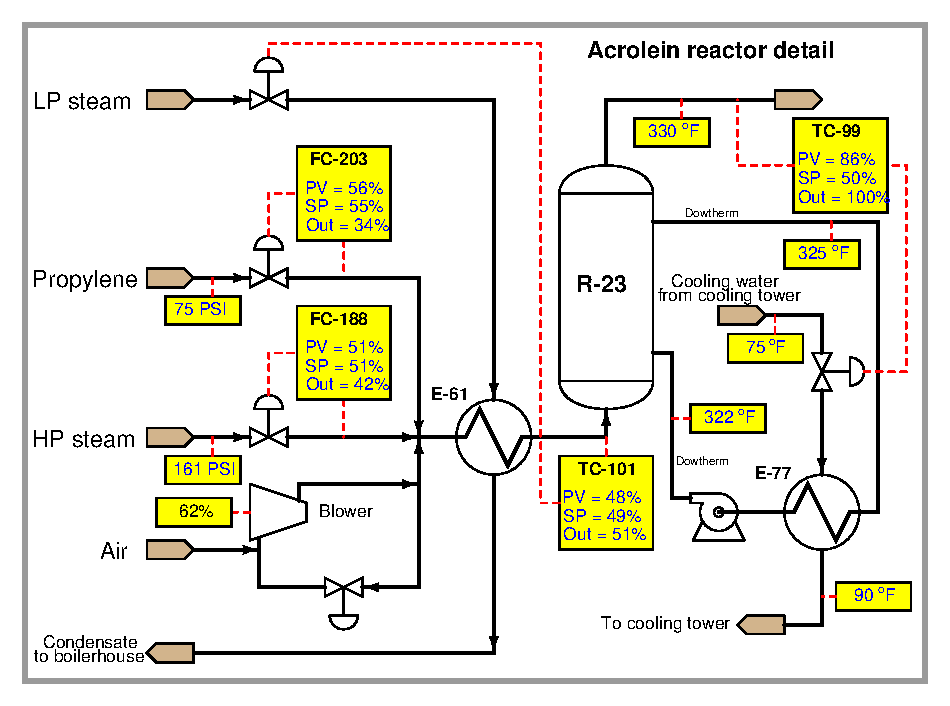
\includegraphics[width=15.5cm]{i00365x01.eps}$$

Reaktoren (R-23) går med altfor høy temperatur. Selv temperaturregulator TC-99 viser utløpstemperatur godt over setpunkt. Operatøren forteller også at han er vant til at Dowtherm-pumpens utløpstemperatur er langt lavere: rundt 260 $^{o}$F i stedet for 322 $^{o}$F. Han sier også at vannet ut fra E-77 til kjøletårnet normalt er betydelig varmere enn 90 $^{o}$F.

\vskip 10pt

Basert på informasjonen i skjermbildet: hjelp operatøren med å identifisere mest sannsynlig årsak til overopphetet reaktor (fra listen under), og forklar hvorfor du valgte akkurat det svaret:

\begin{itemize}
\item{} Reguleringsventil TV-101 sitter mekanisk fast i full åpen stilling
\item{} Kjøletårn for vann er slått av (kjøler ikke nok)
\item{} Varmeveksler E-61 har dårlig varmeoverføring på grunn av ``fouling'' i rør
\item{} Reguleringsventil TV-99 sitter mekanisk fast åpen
\item{} Varmeveksler E-77 har dårlig varmeoverføring på grunn av ``fouling'' i rør
\item{} Reguleringsventil TV-99 sitter mekanisk fast lukket
\item{} Regulator TC-99 står i manuell modus
\item{} Dowtherm-pumpen går for raskt (for stor flow)
\end{itemize}

\filbreak


\underbar{file i00365}
%(END_QUESTION)





%(BEGIN_ANSWER)

{\bf Varmeveksler E-77 med dårlig varmeoverføring pga. ``fouling'' i rørene} er den mest sannsynlige årsaken blant alternativene. Dette forklarer både for høy Dowtherm-utløpstemperatur og hvorfor kjølevann ut av denne veksleren ikke er særlig varmt sammenlignet med innløpstemperaturen.

At TV-99 sitter fast lukket kan også forklare høy Dowtherm-temperatur, fordi dette kan føre til at kjølevann koker ut av E-77 og til slutt gir null flow i utgående linje. Da kan denne linjen kjøles ned og muligens vise 90 grader, slik den gjør her.

\vskip 10pt

5 poeng for riktig valg, 5 poeng for logisk forklaring.

%(END_ANSWER)





%(BEGIN_NOTES)

{\bf Denne oppgaven er ment for eksamen og ikke for arbeidsark!}.

%INDEX% Process: acrolein production

%(END_NOTES)
